%%%%%%%%%%%%%%%%%%%%%%%%%%%%%%%%%%%%%%%%%
% Beamer Presentation
% LaTeX Template
% Version 1.0 (10/11/12)
%
% This template has been downloaded from:
% http://www.LaTeXTemplates.com
%
% License:
% CC BY-NC-SA 3.0 (http://creativecommons.org/licenses/by-nc-sa/3.0/)
%
%%%%%%%%%%%%%%%%%%%%%%%%%%%%%%%%%%%%%%%%%

%----------------------------------------------------------------------------------------
%	PACKAGES AND THEMES
%----------------------------------------------------------------------------------------

\documentclass{beamer}

\mode<presentation> {

% The Beamer class comes with a number of default slide themes
% which change the colors and layouts of slides. Below this is a list
% of all the themes, uncomment each in turn to see what they look like.

%\usetheme{default}
%\usetheme{AnnArbor}
%\usetheme{Antibes}
%\usetheme{Bergen}
%\usetheme{Berkeley}
%\usetheme{Berlin}
\usetheme{Boadilla}
%\usetheme{CambridgeUS}
%\usetheme{Copenhagen}
%\usetheme{Darmstadt}
%\usetheme{Dresden}
%\usetheme{Frankfurt}
%\usetheme{Goettingen}
%\usetheme{Hannover}
%\usetheme{Ilmenau}
%\usetheme{JuanLesPins}
%\usetheme{Luebeck}
%\usetheme{Madrid}
%\usetheme{Malmoe}
%\usetheme{Marburg}
%\usetheme{Montpellier}
%\usetheme{PaloAlto}
%\usetheme{Pittsburgh}
%\usetheme{Rochester}
%\usetheme{Singapore}
%\usetheme{Szeged}
%\usetheme{Warsaw}

% As well as themes, the Beamer class has a number of color themes
% for any slide theme. Uncomment each of these in turn to see how it
% changes the colors of your current slide theme.

%\usecolortheme{albatross}
%\usecolortheme{beaver}
%\usecolortheme{beetle}
%\usecolortheme{crane}
%\usecolortheme{dolphin}
%\usecolortheme{dove}
%\usecolortheme{fly}
%\usecolortheme{lily}
%\usecolortheme{orchid}
%\usecolortheme{rose}
%\usecolortheme{seagull}
%\usecolortheme{seahorse}
%\usecolortheme{whale}
%\usecolortheme{wolverine}

%\setbeamertemplate{footline} % To remove the footer line in all slides uncomment this line
%\setbeamertemplate{footline}[page number] % To replace the footer line in all slides with a simple slide count uncomment this line

\setbeamertemplate{navigation symbols}{} % To remove the navigation symbols from the bottom of all slides uncomment this line
}

\usepackage{amsmath}
\usepackage{amsfonts,amssymb,mathrsfs, bm}
\usepackage{amsbsy}
\usepackage[absolute,overlay]{textpos}
\usepackage{appendixnumberbeamer}
\setbeamercolor{framesource}{fg=gray}
\setbeamerfont{framesource}{size=\tiny}
 \usepackage[labelformat=empty,font=scriptsize,skip=0pt,justification=justified,singlelinecheck=false]{caption}


\newcommand{\source}[1]{\begin{textblock*}{6cm}(0cm,8.6cm)
    \begin{beamercolorbox}[ht=0.5cm,right]{framesource}
        \usebeamerfont{framesource}\usebeamercolor[fg]{framesource} {#1}
    \end{beamercolorbox}
\end{textblock*}}

%----------------------------------------------------------------------------------------
%	TITLE PAGE
%----------------------------------------------------------------------------------------

\title[]{Association of Neural Activity with Response to Dietary Regimine 
for Treatment of Depression} % The short title appears at the bottom of every slide, the full title is only on the title page

\author{Maime Guan, Lingge Li, Duy Ngo, \\Fulya Ozcan, Dustin Pluta, Yuxiao Wang} % Your name
\institute[UCI] % Your institution as it will appear on the bottom of every slide, may be shorthand to save space
{
 \\ % Your institution for the title page
\medskip
\textit{} % Your email address
}
\date{\today} % Date, can be changed to a custom date



\begin{document}

\begin{frame}
\titlepage % Print the title page as the first slide
\end{frame}


\section*{Overview}

\begin{frame}
\tableofcontents
\end{frame}


\section{Background}

\begin{frame}
\frametitle{Motivating Questions}
\begin{itemize}
\item Is SPECT brain imaging predictive of response to treatment of depression through a dietary regimine?
\item Are there specific brain regions associated with response to treatment?
\item How does the association of brain activation with treatment response differ across to demographic subgroups?
\end{itemize}
\end{frame}


\begin{frame}
\frametitle{Project Goals}
\begin{itemize}
\item Build a model to predict treatment response from SPECT imaging and clinical covariates.
\item Test the strength of association between brain activation and treatment response for selected scientifically relevant brain regions.
\item Identify patient subgroups for which the association of activation with response differs
\end{itemize}
\end{frame}

\begin{frame}
\frametitle{Background}
\begin{itemize}
\item SPECT uses a radioactive tracer to measure cerebral blood flow.
\item A 3D map of the brain is produced, indicating areas of high activity and low activity.
\item Results of previous studies using SPECT:
\begin{itemize}
\item Distinguish traumatic brain injury (TBI) cases from post-traumatic stress disorder cases with high accuracy (Raji 2015).
\item Distinguish NFL players with repeated head trauma from healthy population (Amen 2016).
\item Distinguish autism spectrum disorder from healthy subjects (Amen 2016).
\end{itemize}
\end{itemize}
\end{frame}

\begin{frame}
\frametitle{Background}
\textbf{A SPECT Scanner}
\begin{center}
\begin{figure}
\includegraphics[scale=0.2]{SPECT_CT}
\end{figure}
\end{center}
\end{frame}

\begin{frame}
\frametitle{Background}
\textbf{A SPECT Image}
\begin{center}
\begin{figure}
\includegraphics[scale=0.45]{SPECT}
\end{figure}
\end{center}
\end{frame}

\section{Data Description}

\begin{frame}
\frametitle{Data Description}
\textbf{Patients}
\begin{enumerate}
\item 828 patients diagnosed with depression.  Most patients had a history of various mental illnesses or disorders, and were typically not responsive to traditional treatments before being referred to Dr. Amen's clinic.
\item Basic demographic information was collected for all patients.
\item Patients were given preliminary clinical exams to assess any medical conditions, and any co-diagnoses recorded.
\item Single Photon Emission Computed Tomography (SPECT) scans were also collected for all patients during the initial exam.
\end{enumerate}
\end{frame}

\begin{frame}
\frametitle{Data Description}
\textbf{Response Values}
\begin{enumerate}
\item  During the initial exam, patients were given the Beck Depression Inventory (BDI) survey to measure level of depression.
\item Each patient was asked to follow a dietary regimine of supplements and vitamins designed to naturally treat depression and other disorders.
\item After 5-7 months of dietary treatment patients were given a follow-up BDI survey.
\item "Raw" response values are taken as 
\[\Delta\textit{BDI} = \textit{Pre\_BDI} - \textit{Post\_BDI}\]
\item These values were then dichotomized into \textit{Responders} and \textit{Non-responders}.
\end{enumerate}
\end{frame}

\begin{frame}{Data Description}
\begin{center}
\includegraphics[scale=0.5]{BDI_hist}
\end{center}
\end{frame}

\begin{frame}{Who are the responders}
In the original data, patients with BDI less than 25 prior to treatment were all labeled as non-responders. Our models were able to get above $60\%$ accuracy but they were actually only finding patients with low BDI. Therefore, we changed the labels as one would expect.
\begin{figure}[H]
\includegraphics[width=0.52\textwidth]{responder.png}
\includegraphics[width=0.52\textwidth]{full.png}
\end{figure}
\end{frame}

\begin{frame}{Data Description}
\centering
\begin{table}
\begin{tabular}{lcc}
\hline
\textbf{Covariate}& \textbf{N (\%)} & \textbf{Mean BDI\_Change }\\\hline\hline
\textbf{Gender }& & \\
\hspace{0.1in} Male & 460 (0.56) & -15.26\\
\hspace{0.1in} Female & 368 (0.44) & -14.86\\
\textbf{Age Group }& & \\
\hspace{0.1in} Pediatric & 14 (0.02) & -14.68\\
\hspace{0.1in} Adult & 753 (0.91) & -15.13\\
\hspace{0.1in} Geriatric & 61 (0.07) & -14.02\\
\textbf{Co-diagnosis}& & \\
\hspace{0.1in} ADHD & 439 & -14.98\\
\hspace{0.1in} Anxiety & 631 & -14.89\\
\hspace{0.1in} Bipolar & 71 & -15.35\\
\hline
\end{tabular}
\end{table}
\end{frame}

\begin{frame}{Basic Predictive Modelling}
We tried logistic regression with $L1$ penalty, support vector machine, and boosted trees. However, they performed barely better than tossing a coin. 
\begin{figure}[H]
\includegraphics[width=0.48\textwidth]{accuracy.png}
\includegraphics[width=0.48\textwidth]{auc.png}
\caption{Cross validation LASSO results}
\end{figure}
\end{frame}


\section{Exploratory Analysis}
\begin{frame}
\frametitle{Exploratory Analysis}
\begin{center}
\includegraphics[scale=0.5]{subject_activation}
\end{center}
\end{frame}

\begin{frame}
\frametitle{Exploratory Analysis}
\begin{center}
\includegraphics[scale=0.5]{roi_activation}
\end{center}
\end{frame}

\begin{frame}
\frametitle{Exploratory Analysis}
\begin{overprint}
\only<1>{
\begin{itemize}
\item Number of subject: 1041. Number of brain region: 256. 
\end{itemize}
\begin{center}
\includegraphics[width=12.5cm,height=8cm]{Figures/boxplot}\\
\end{center}
}
\end{overprint}
\end{frame}

\begin{frame}
\frametitle{Clustering Analysis: Hierarchical Tree}
\begin{overprint}
\only<1>{
\begin{itemize}
\item Hierarchical tree (dendrogram) for all subjects. 
\end{itemize}
\begin{center}
\includegraphics[width=13cm,height=7cm]{Figures/Dendrogram}\\
\end{center}
}

\only<2>{
\begin{itemize}
\item Number of cluster = 2
\end{itemize}
\begin{center}
\includegraphics[width=13cm,height=7cm]{Figures/Numbercluster2}\\
\end{center}
}

\only<3>{
\begin{itemize}
\item Number of cluster = 3
\end{itemize}
\begin{center}
\includegraphics[width=13cm,height=7cm]{Figures/Numbercluster3}\\
\end{center}
}

\only<4>{
\begin{itemize}
\item Number of cluster = 4 and so on.
\end{itemize}
\begin{center}
\includegraphics[width=13cm,height=7cm]{Figures/Numbercluster4}\\
\end{center}
}
\end{overprint}
\end{frame}

\begin{frame}
\frametitle{Clustering Analysis: K-Mean}
\begin{overprint}
\only<1>{
\begin{itemize}
\item Decide number of cluster based on the percentage of variance explained as a function of the number of clusters 
\end{itemize}
\begin{center}
\includegraphics[width=12cm,height=7cm]{Figures/KMeanValid}
\end{center}
}

\only<2>{
\begin{itemize}
\item Number of cluster = 3. 
\end{itemize}
\begin{center}
\includegraphics[width=12cm,height=7cm]{Figures/KMeanVisualize}\\
\end{center}
}

\only<3>{
\begin{tabular}{cc}
Number of cluster = 2 &  Number of cluster = 4 \\
\includegraphics[width=5.8cm,height=6cm]{Figures/KMeanVisualize2} & \includegraphics[width=5.8cm,height=6cm]{Figures/KMeanVisualize4} \\
\end{tabular}
}
\end{overprint}
\end{frame}

\section{Feature Reduction}

\begin{frame}\frametitle{Feature Reduction}
\begin{block}{Challenges}
\begin{itemize}
\item 954 observations, 1654 possible features, 11 main feature groups
\item Missing data (especially for certain group of features)
	\end{itemize}\end{block}
\begin{block}{Step-0: Feature Reduction Using All Possible Features}
	\begin{itemize}
	\item 	Top 5 features: ``Pre\_GSI",``PRE\_PST",``Pre\_PSDI",``Pre\_BDI",``Baseline\_location"\end{itemize}
	\begin{figure}[ht]
\includegraphics[width=4.2in,height=1.4in]{rfe_results_all.pdf}	\end{figure}	
\end{block}	
\end{frame}

\begin{frame}\frametitle{Feature Reduction}

	\begin{block}{Step-1: Grouping Features}
		\begin{itemize}
			\item 11 feature groups:
			\begin{itemize}
				\item Demographics, Comorbidities, T Baseline, T Concentration, Baseline, Concentration, max cluster size, min cluster size, max cluster T Baseline, min cluster T Baseline
				
			\end{itemize}
	\end{itemize}\end{block}	\begin{block}{Step-2: Imputation}
\begin{enumerate}
\item Remove columns with more than a certain threshold of missing values
\item Impute the remaining missing values using Gelman's \textbf{mi} package
\end{enumerate}\end{block}	
\end{frame}


\begin{frame}\frametitle{Feature Reduction}

\begin{figure}[ht]
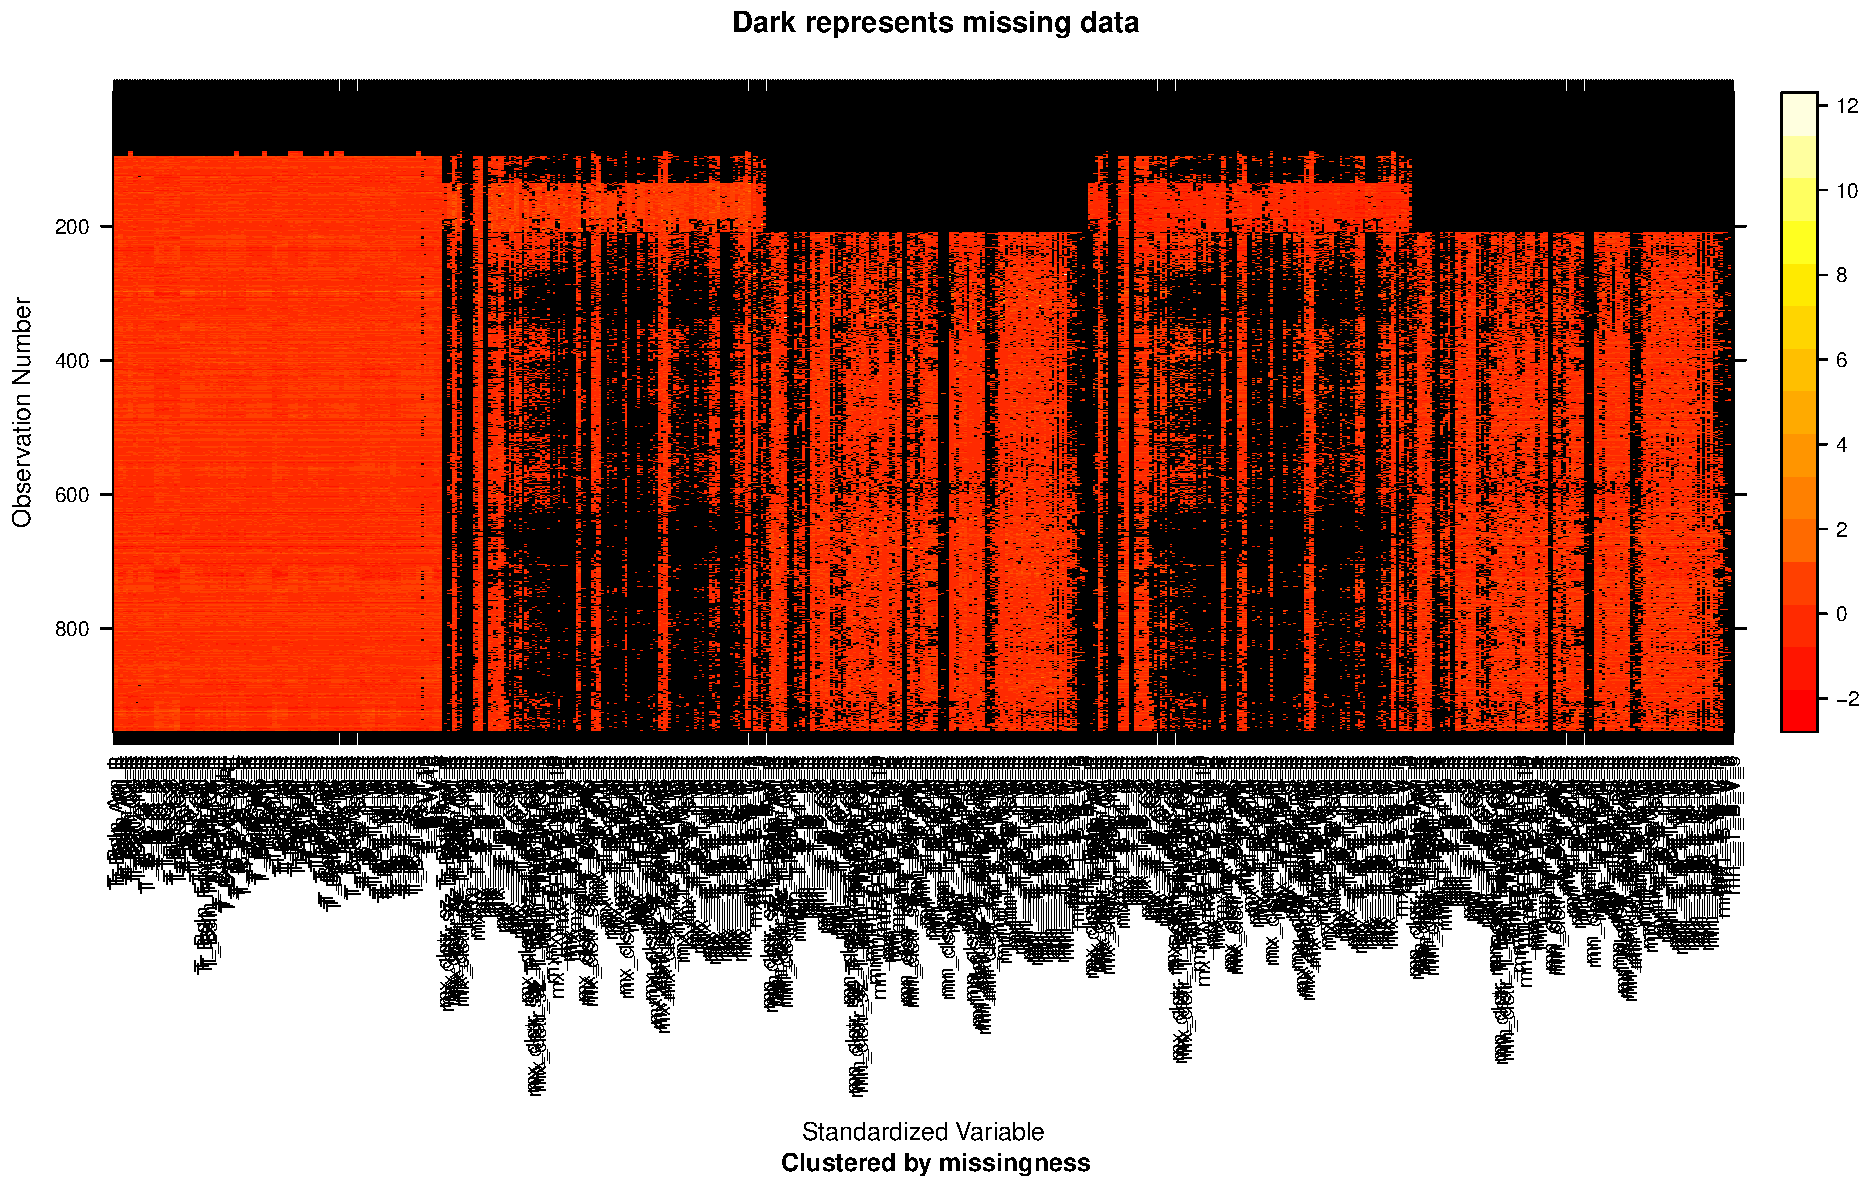
\includegraphics[width=4.8in,height=4in]{missing.pdf}
\caption{\footnotesize Columns with missing values in T Baseline group}
	\end{figure}	\end{frame}
		
\begin{frame}\frametitle{Feature Reduction}
	\begin{block}{Step-3: Imputation}
		\begin{enumerate}
			\item Remove columns with more than a certain threshold of missing values
			\item Impute the remaining missing values using Gelman's \textbf{mi} package
		\end{enumerate}\end{block}
	\begin{block}{Step-4: K-means within feature groups and outcome }
		\begin{enumerate}
			\item  K-means on comorbidities 
			\item  K-means on groups
		\end{enumerate}\end{block}
			\end{frame}	
			
\begin{frame}\frametitle{Feature Reduction}
	\begin{block}{Step-5: Overall Feature Reduction-Recursive Feature Elimination}
		\begin{enumerate}
			\item Constructs an Learning Vector Quantization (LVQ) 
			\item Variable importance is estimated for each group
			\item Most important variables are merged in a new feature matrix 
			\item  Number of features reduced from 1655 to 652 
		\end{enumerate}\end{block}\begin{block}{Step-6: Logistic Regression to find significant variables}
	\begin{itemize}
	\item Number of features reduced from 652 to 94
\end{itemize}\end{block}			
	\end{frame}	

\begin{frame}
	\begin{figure}[ht]\frametitle{Feature Reduction}
		\includegraphics[width=4.6in,height=4.2in]{significant_list.pdf}

	\end{figure}
\end{frame}	

%------------------------------------------------
\section{Bayesian Logistic Regression} 

%------------------------------------------------

\begin{frame}
\frametitle{Bayesian Logistic Regression}
Still has the same components:
\begin{enumerate}
\item Random: $Y_{i} \sim Bernoulli \left( p_{i} \right) $
\item Systematic and link: $ \log \left( \frac{p_{i}}{1-p_{i}} \right) = \beta_{0} + \beta_{1}X_{1i} + \beta_{2}X_{2i} + \beta_{3}X_{3i} + \ldots $
\end{enumerate}

To estimate the $\beta_{k}$'s in a Bayesian framework, we define priors for the coefficients of the predictors. Using a multivariate normal prior for $\beta_{k}$:
\medskip
\begin{center}
$ \beta_{k} \sim MVN \left( \mu = 0, 1/\sigma^{2} = .0001  \right), k = 1,2, \ldots $
\end{center}

Can be implemented with 'MCMCpack' or bayesglm (from 'arm' library) in R, or with JAGS.

\end{frame}

%------------------------------------------------

\begin{frame}

\frametitle{Bayesian Logistic Regression}
Models tried so far:
\begin{itemize}
\item Using \emph{all 128 brain regions} as predictors (chains did not converge).
\item Using brain regions known to be \emph{associated with depression}: amygdala, hippocampus, thalamus, and insula. (prediction = 52.5\%)
\item Using some \emph{comorbidities} of interest (anxiety, ADHD, substance abuse, frontal lobe dysfunction, brain trauma, and PTSD) with \emph{compliance score}. (prediction = 51.5\%)
\item Using some comorbodities, compliance score, and brain regions associated with depression. (prediction = 54.5\%)
\end{itemize}
\medskip
Cross-validation with 828 patients in training set and 200 patients in test set.

\end{frame}

%------------------------------------------------

\begin{frame}
This is quite representative of the findings for the brain regions: posterior samples of coefficients mostly right about 0 \ldots

\begin{figure}
\includegraphics[width=0.7\linewidth]{figure_posteriorAmygdala}
\end{figure}

\end{frame}

%------------------------------------------------

\begin{frame}
However, some coefficients may be more interesting \ldots

\begin{figure}
\includegraphics[width=0.7\linewidth]{figure_posteriorAnxiety}
\end{figure}
About a predicted 40\% decrease in the odds of responding to treatment if a patient has anxiety as well as depression, compared to not having anxiety.

\end{frame}

%------------------------------------------------

\begin{frame}
However, some coefficients may be more interesting \ldots

\begin{figure}
\includegraphics[width=0.7\linewidth]{figure_posteriorNotCompliant}
\end{figure}
About a predicted 63\% decrease in the odds of responding to treatment if a patient self-reported being "not compliant", compared to not answering.

\end{frame}


\section{Next Steps}
\begin{frame}
\frametitle{Next Steps}
So far, we have only tried Bayesian logistic regression, where all the predictors are directly related to the odds of response to treatment.

\begin{figure}
\includegraphics[width=0.7\linewidth]{figureBayesLR}
\end{figure}

\end{frame}

%------------------------------------------------

\begin{frame}
\frametitle{Next Steps}
We can also try different underlying structures, defining other possible relationships between variables. For example:

\begin{figure}
\includegraphics[width=0.7\linewidth]{figureSEM}
\end{figure}
\end{frame}

\begin{frame}{Next Steps}
\begin{enumerate}
\item Select a dimension reduction method for SPECT covariates.
\item Build, validate, and interpret models for hypothesis testing.
\item Tune and compare prediction models.
\end{enumerate}
\end{frame}


\section{Summary}
\begin{frame}{Summary}
\begin{itemize}
\item Exploratory analyses and preliminary modeling suggest that separating Responders from Non-responders is difficult from the available covariates.
\begin{itemize}
\item This is a more challenging setting than previous studies since we are classifying within Depression patient subgroup, instead of separating cases from controls.
\end{itemize}
\item There is some weak clustering by SPECT imaging, but these clusters aren't strongly associated with change in BDI.  Supervised dimension reduction methods may give better groupings.
\end{itemize}
\end{frame}

\begin{frame}
\centering
\Large
\textbf{Thanks!}
\end{frame}

\end{document}















